% !TEX program = pdflatex
\documentclass[11pt,xcolor={dvipsnames}]{beamer} % presentation output
% \documentclass[11pt,xcolor={dvipsnames},handout]{beamer} % Beamer printout
% xcolor allows to use many new colors with \usecolortheme

\mode<presentation>{
  \usetheme{Warsaw}
%  Here is a gallery with other themes:
%  http://deic.uab.es/~iblanes/beamer_gallery/
  \usecolortheme[named=OliveGreen]{structure}
%  Others: OliveGreen, Brown, Sepia, RawSienna,
  \useoutertheme{shadow}
 	\setbeamercovered{transparent}
	\setbeamercolor{block title example}{fg=white,bg=Blue}
	\setbeamercolor{block body example}{fg=black,bg=Blue!10}
	\setbeamercolor{postit}{fg=black,bg=OliveGreen!20}
	\setbeamercolor{postit2}{fg=yellow,bg=OliveGreen}
%    \setbeamercolor{NEW_STYLE_NAME}{fg=COLOR_FOREGROUNG,bg=COLOR_BACKGROUNG}
}

%% Setting for Beamer printout
% reference: http://mathoverflow.net/questions/5893/beamer-printout
\usepackage{pgfpages}
\mode<handout>{
  \usetheme{default}
  \setbeamercolor{background canvas}{bg=Black!5}
  \pgfpagesuselayout{4 on 1}[a4paper,portrait,border shrink=2.5mm]
  % 4 slide in one page
}
%% Setting for Beamer printout

\usepackage[italian]{babel}
\usepackage[latin1]{inputenc}
\usepackage{times}
\usepackage[T1]{fontenc}
\usepackage{graphics}
\graphicspath{{images/}}
% all the graphics files will go in the subdirectory images
\usepackage{numprint}
% with this one \np{1000} becomes 1 000
\usepackage{mathcomp}
\usepackage{gensymb}
% with this one \numprint[\textcelsius]{20} becomes 20�C
\newcommand{\ud}{\mathop{}\ \mathrm{d}}
% with this one \ud{x} becomes dx
\usepackage{mathtools}
\DeclarePairedDelimiter{\abs}{\lvert}{\rvert}
% to define absolute value (mathtools is required)

\hypersetup{
			pdftitle={Workshop},
			pdfsubject={Git Workshop},
			pdfauthor={Mojtaba Goodarzi},
			pdfkeywords={GIT},
			pdfpagemode=FullScreen, % once opened it goes in fullscreen modality
			%citecolor=black,
			%filecolor=black,
			%linkcolor=black,
			%urlcolor=black
}

\usepackage[absolute,overlay]{textpos}
\setlength{\TPHorizModule}{1mm}
\setlength{\TPVertModule}{1mm}

%%%% A NEW COMMAND TO FIX LOGO POSITION (x,y) in mm
\newcommand{\MyLogo}{%
\begin{textblock}{14}(2.0,0.1)
%  \pgfuseimage{logo}
 
\includegraphics[height=1cm, angle=0]{logo}
\end{textblock}
}
%%%% A NEW COMMAND TO FIX LOGO POSITION (x,y) in mm

%%%%%%%%%%%%%%%%%%%%%%%%%%%%%%%%%%%%%%%%%%%%%%%%%%%%%%%%%%%%%%%%%%%%%%%%%

\title[Git workshop]{Git workshop}
\author[Mojtaba Goodarzi]
{Mojtaba Goodarzi}
\institute[Sepehr]
{
  Sepehr
  }
\date{September 26, 2021}

%\logo{
\includegraphics[height=1.5cm, angle=0]{logo}}
% To have a logo on each page... BAD RESULT!!

%\titlegraphic{
\includegraphics[height=1.4cm, angle=0]{logo}}
% To have an imagie on title page

%%%% TO HAVE A TOC ON EVERY SLIDE
%\AtBeginSubsection[]
%{
%  \begin{frame}<beamer>{Sommario}
%    \tableofcontents[currentsection,currentsubsection]
%    \tableofcontents[currentsection]
%    \tableofcontents
%  \end{frame}
%}
%%%% TO HAVE A TOC ON EVERY SLIDE

\begin{document}
\transduration{1}

%%%%%%%%%%%%%%%%%%%%%%%%%%%%%    TITLE    %%%%%%%%%%%%%%%%%%%%%%%%%%%%%%%
\begin{frame}
	\MyLogo
	\begin{center}
		% \includegraphics[height=1.5cm, angle=0]{unipd}
		\titlepage
	\end{center}
\end{frame}

%%%% TOC
%\begin{frame}{Contents}
%\MyLogo
%\tableofcontents[pausesections,part=1]
%  \tableofcontents
%\end{frame}



%%%%%%%%%%%%%%%%%%%%%%%%%%%% FIRST SECTION %%%%%%%%%%%%%%%%%%%%%%%%%%%%%%
\section{GIT}

\begin{frame}
	%\transblindshorizontal
	% type of transition effect

	
\includegraphics[height=300px]{why-git.png}
\end{frame}

\begin{frame}
	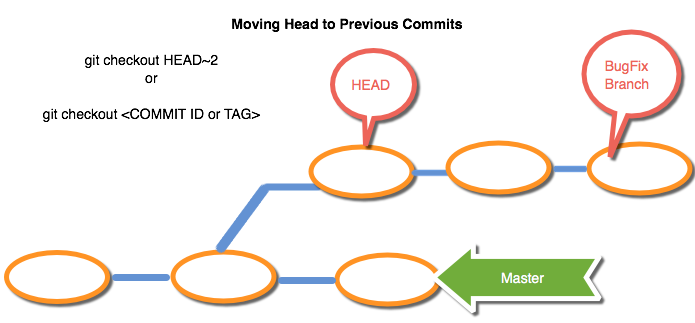
\includegraphics[height=250px,width=300px]{git-checkout.png}
\end{frame}

\begin{frame}
	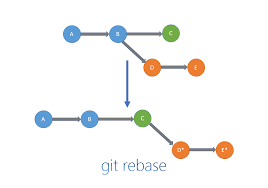
\includegraphics{rebase.png}
\end{frame}

\begin{frame}
	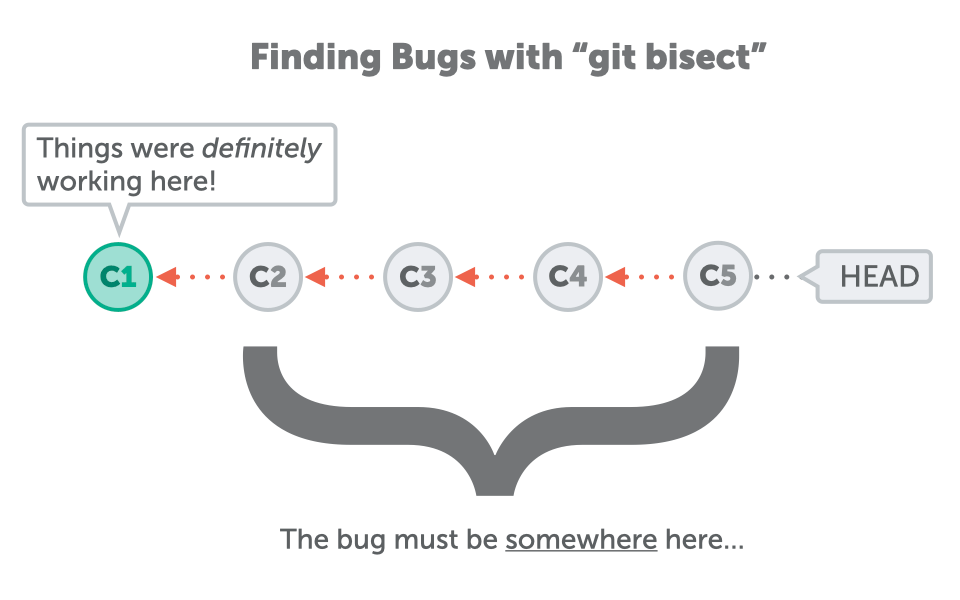
\includegraphics[height=250px,width=300px]{bisect-overview.png}
\end{frame}

\begin{frame}
	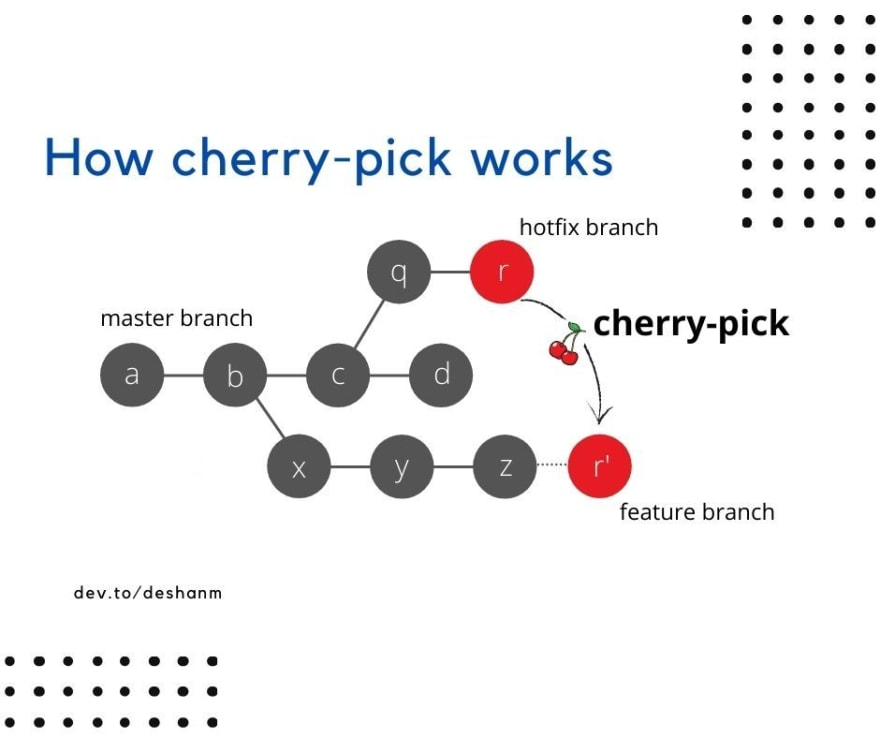
\includegraphics[height=250px,width=300px]{cherry-pick.jpg}
\end{frame}

\begin{frame}
	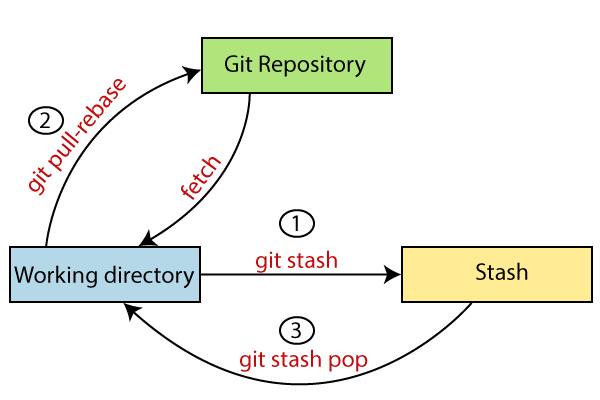
\includegraphics[height=250px,width=300px]{git-stash.png}
\end{frame}

\begin{frame}
	\begin{block}{git clean}
		\begin{itemize}
			\item git clean -f     \# remove untracked files
			\item git clean -fd    \# remove untracked files/directories
			\item git clean -nfd   \# list all files/directories that would be removed
		\end{itemize}
	\end{block}
\end{frame}

\begin{frame}
	\begin{block}{git cat-file}
		\begin{itemize}
			\item git cat-file -t    \# display type of the object
			\item git cat-file -p    \# display content of the object
		\end{itemize}
	\end{block}
\end{frame}

\begin{frame}
	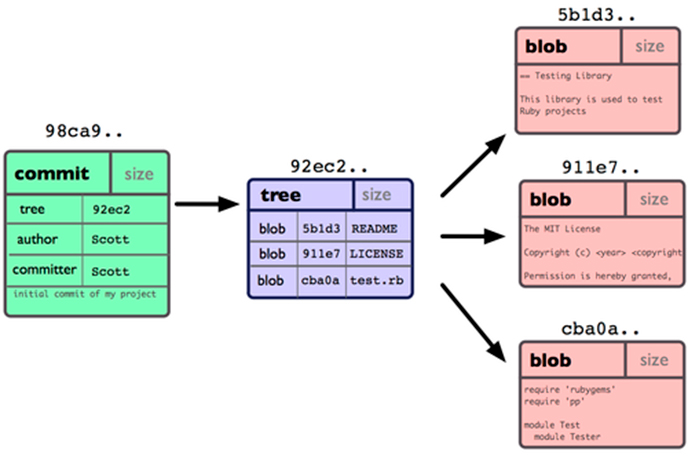
\includegraphics[height=250px,width=300px]{git-blobs.jpg}
\end{frame}

\begin{frame}
	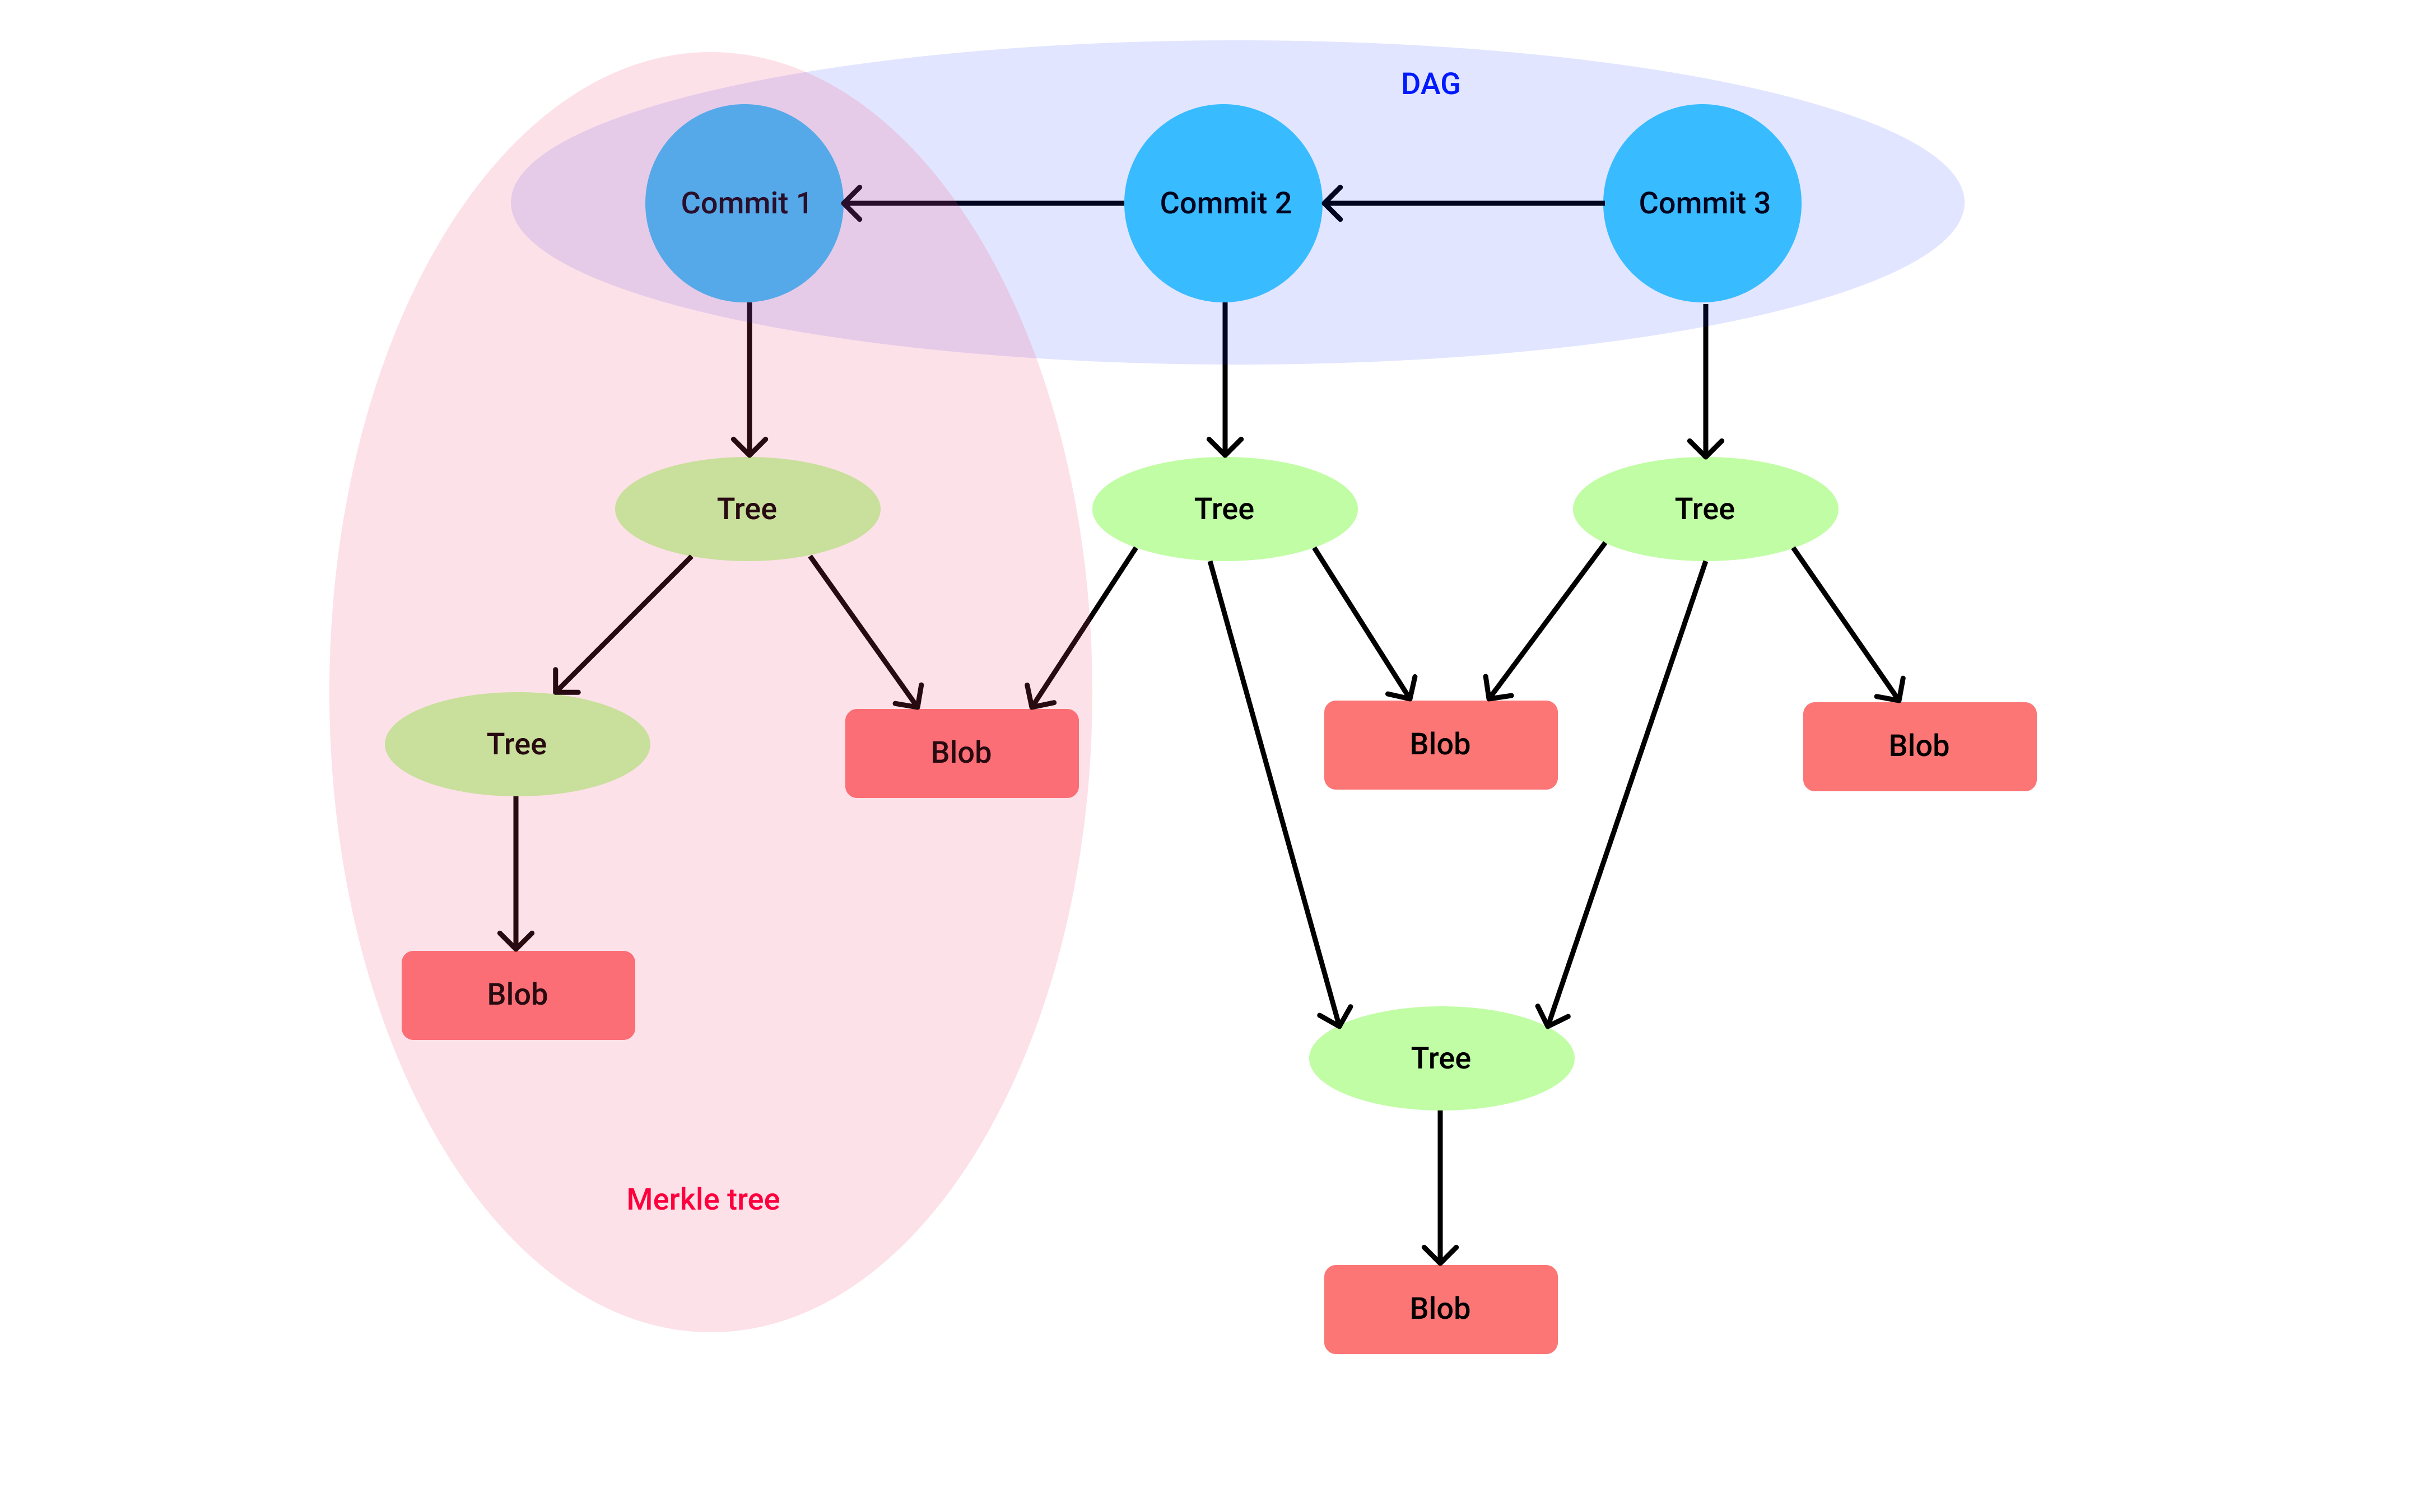
\includegraphics[height=250px,width=300px]{commit-graph.png}
\end{frame}
%%%%%%%%%%%%%%%%%%%%%%%%%%%%%% LAST FRAME %%%%%%%%%%%%%%%%%%%%%%%%%%%%%%%
\begin{frame}
	\transboxin
	\MyLogo
	\vspace{1.0cm}
	\begin{beamercolorbox}[sep=1.0cm, center, shadow=false, rounded=true]{postit2}
		\begin{Huge}Many Thanks\end{Huge}
	\end{beamercolorbox}
\end{frame}

\end{document}